\section{Цел на теста}

Целта на теста е проверка на придобитите знания и умения на ученици в 8-ми клас във несъществуващо училище, свързани с подтемата "Приложни програми" от задължителната учебна програма, както и установяване на наличието на затруднения по разглежданата тема.

\section{Съдържателна рамка}

\subsection{Съдържателни области}

\begin{enumerate}
    \item Текстообработващи програми:
          \subitem Основни възможности за използване на шаблони.
          \subitem Работа с готови шаблони в различни режими.
          \subitem Създаване на шаблон за текстов документ.
          \subitem Стандартни теми на документи и създаване на собствена тема.
          \subitem Създаване на циркулярни писма.
          \subitem Свързване на циркулярно писмо със създаден списък.
          \subitem Ползване и създаване на формуляри.
    \item Електронни таблици:
          \subitem Проектиране и попълване на електронна таблица за съхраняване на атрибутите на конкретен обект.
          \subitem Налагане на ограничения на въвежданите данни.
          \subitem Изготвяне на справки по критерии за търсене.
          \subitem Обобщаване на данни по определен критерий.
          \subitem Дизайн на формуляри.
          \subitem Филтриране на данни чрез комбинирани заявки.
          \subitem Валидиране на данни.
          \subitem Междинни пресмятания в подредени таблици.
\end{enumerate}

\subsection{Познавателни области}
\begin{enumerate}
    \item Знание и разбиране:
          \subitem Познаване на основните възможности на текстообработващите програми и електронните таблици.
          \subitem Разбиране на понятията, свързани с шаблони, теми на документи, циркулярни писма, и формуляри.
          \subitem Познаване на начините за създаване и използване на шаблони, циркулярни писма и формуляри.

    \item Приложение:
          \subitem Използване на изучаваните функции и инструменти за създаване и модифициране на текстови документи и електронни таблици.
          \subitem Приложение на различни методи за създаване на шаблони и теми, проектиране и попълване на електронни таблици, налагане на ограничения и валидиране на данни.
          \subitem Решаване на практически задачи чрез изготвяне на справки и обобщаване на данни.

    \item Анализиране и моделиране:
          \subitem Анализ на ситуациите и изискванията за създаване и използване на документи и електронни таблици.
          \subitem Моделиране на реални ситуации чрез проектиране на формуляри и електронни таблици, валидиране на данни и извършване на междинни пресмятания.
          \subitem Решаване на практически казуси чрез комбиниране на различни функции и инструменти в текстообработващите програми и електронните таблици.
\end{enumerate}

\section{Структура на теста}

\subsection{Вид и времетраене}

Тестът е предвиден за полагане в писмен вид. Това ще се случи в рамките на един учебен час, чиято продължителност е 40 минути.

\subsection{Формат}
Тестът се състои от 16 задачи с избираем отговор. Към всяка задача са предоставени 4 възможни отговора, от които точно един е верен.

Отбелязването на верен отговор се оценява с 1 точка. При отбелязан грешен отговор или при липсата на отбелязан такъв, съответната задача ще се оценява с 0 точки, т.е. не повлиява по негативен начин.

\section{Тестова спецификация}
\begin{figure}[H]
    \centering
    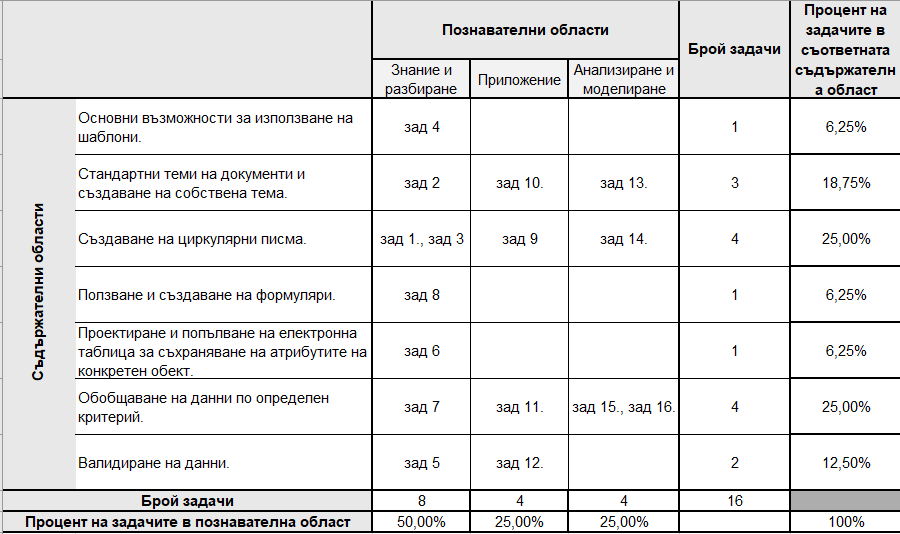
\includegraphics[width=\linewidth]{resources/category-of-problems.png}
    \caption{Тестова спецификация}
\end{figure}

\section{Инструкции за работа}
Тестът се състои от 16 задачи с избираем отговор. Всяка задача има 4 възможни отговора, от които точно един е верен. Отбелязването на верен отговор носи 1 точка, а отбелязването на грешен отговор или оставянето на задача без отговор носи 0 точки.

За да отбележите своя отговор, зачертайте със знака X буквата на избрания от Вас отговор. Ако решите, че първоначалният Ви отговор не е верен, запълнете кръгчето с грешния отговор и зачертайте със знака X буквата на друг отговор, който смятате за верен.

Време за работа – 40 минути.
Успешна работа!

\newpage
\section{Тест}
\begin{center} \Large
    Контролна работа \\
    Приложни програми
\end{center}
Име ........................................................................... Клас ........... №............

% Текстообработващи програми
% Знание и разбиране
% 
зад 1. /1т./ Коя опция в текстообработващите програми се използва за създаване на циркулярно писмо?\\
а) Файл > Отвори\\
б) Вмъкване > Циркулярно писмо\\
в) Пощенски съобщения > Създай циркулярни писма\\
г) Форматиране > Циркулярно писмо\\

% 
зад 2. /1т./ Коя функция се използва за създаване на нов шаблон в текстов документ?\\
а) Файл > Запиши като шаблон\\
б) Вмъкване > Шаблон\\
в) Изглед > Шаблон\\
г) Инструменти > Шаблон\\

% 
зад 3. /1т./ Как се нарича процесът на свързване на циркулярно писмо със списък с адресати?\\
а) Сливане\\
б) Комбиниране\\
в) Обединяване\\
г) Свързване\\

% 
% 
зад 4. /1т./ Коя от следните опции се използва за създаване на нова тема на документ в текстообработваща програма?\\
а) Вмъкване > Тема\\
б) Форматиране > Тема\\
в) Дизайн > Тема\\
г) Файл > Тема\\

% Електронни таблици 
% Знание и разбиране
% 
зад 5. /1т./ Коя функция в електронните таблици се използва за налагане на ограничения на въведените данни?\\
а) Данни > Филтър\\
б) Формула > Ограничения\\
в) Данни > Проверка на данни\\
г) Редактиране > Ограничения\\

% 
% 
зад 6. /1т./ Коя команда се използва за проектиране на нова електронна таблица?\\
а) Вмъкване > Нова таблица\\
б) Файл > Нова таблица\\
в) Изглед > Таблица\\
г) Данни > Нова таблица\\

% 
зад 7. /1т./ Как се нарича процесът на обобщаване на данни в електронна таблица по определен критерий?\\
а) Филтриране\\
б) Сортиране\\
в) Сумиране\\
г) Групиране\\

% 
зад 8. /1т./ Коя от следните опции позволява създаване на формуляр в електронна таблица?\\
а) Вмъкване > Формуляр\\
б) Данни > Формуляр\\
в) Форматиране > Формуляр\\
г) Файл > Формуляр\\

% Текстообработващи програми
% Приложение
% 
зад 9. /1т./ Кой е правилният начин за създаване на циркулярно писмо в текстообработваща програма?\\
а) Вмъкване на полета и ръчно въвеждане на данни\\
б) Създаване на един документ и отпечатване множество копия\\
в) Използване на функцията за циркулярно писмо и свързване с база данни\\
г) Ръчно копиране и поставяне на информацията във всеки документ\\

% 
зад 10. /1т./ Коя команда се използва за създаване на шаблон за текстов документ?\\
а) Форматиране > Шаблон > Нов \\
б) Файл > Запиши като > Шаблон\\
в) Вмъкване > Шаблон > Нов\\
г) Инструменти > Шаблон > Запиши\\

% Електронни таблици
% Приложение
% 
зад 11. /1т./ Коя опция в електронните таблици се използва за изготвяне на справки по критерии за търсене?\\
а) Филтриране\\
б) Сортиране\\
в) Форматиране\\
г) Проверка на данни\\

% 
зад 12. /1т./ Коя функция се използва за валидиране на данни в електронна таблица?\\
а) Форматиране > Проверка\\
б) Данни > Проверка на данни\\
в) Вмъкване > Ограничения\\
г) Изглед > Проверка \\

% Текстообработващи програми
% Анализиране и моделиране
% 
зад 13. /1т./ Какъв тип шаблон е най-подходящ за създаване на формуляр за анкета?\\
а) Текстов шаблон \\
б) Циркулярен шаблон\\
в) Документен шаблон\\
г) Формуляр шаблон\\

% 
% 
зад 14. /1т./ Коя функция е подходяща за моделиране на бизнес кореспонденция чрез циркулярни писма?\\
а) Вмъкване на таблица \\
б) Създаване на списък с контакти и използване на циркулярно писмо\\
в) Използване на шаблон за бизнес писма\\
г) Създаване на нов документ за всяка кореспонденция\\

% Електронни таблици
% Анализиране и моделиране
% 
зад 15. /1т./ Какъв метод се използва за филтриране на данни чрез комбинирани заявки в електронни таблици?\\
а) Филтриране по един критерий\\
б) Използване на функцията за условно форматиране\\
в) Създаване на сложни филтри с множество критерии\\
г) Ръчно сортиране на данни\\

% 
% 
зад 16. /1т./ Какъв подход е най-подходящ за извършване на междинни пресмятания в подредени таблици?\\
а) Използване на функцията SUM\\
б) Създаване на формула за всяка клетка\\
в) Използване на междинни обобщения\\
г) Ръчно добавяне на стойности\\

\section{Ключ с верни отговори}
\begin{center}
    \begin{tabular}{|c|c|c|c|c|c|c|c|c|c|c|c|c|c|c|c|}
        \hline
        1 & 2 & 3 & 4 & 5 & 6 & 7 & 8 & 9 & 10 & 11 & 12 & 13 & 14 & 15 & 16 \\
        \hline
        в & а & а & в & в & б & г & б & в & б  & а  & б  & г  & б  & в  & в  \\
        \hline
    \end{tabular}
\end{center}

% \section{Тестови карти на задачите}

\section{Апробация}
Отговорите на въпросите са генерирани от Chat GPT, поради невъзможност тестът да бъде апробиран с реални ученици.

\section{Измерителни качества на задачите и теста}
\subsection{Коефициент на трудност}
Коефициентът на трудност на всяка задача измерва каква част от учениците, правили теста, са я решили правилно.
\begin{equation}
    C_\text{трудност} = \frac{\text{отговорили вярно}}{\text{решавали задачата}}
\end{equation}
Очевидно $C_\text{трудност} \in [0; 1]$.

Ако $C_\text{трудност} \approx 1$, то задачата е лесна. Обратно, ако $C_\text{трудност} \approx 0$ - задачата е трудна.
\begin{itemize}
    \item Много лесни - 7, 9, 13, 16
    \item Лесни - 4, 5, 6, 8, 10, 11
    \item Оптимани - 1, 2
    \item Трудни - няма
    \item Много трудни - 3, 12, 14, 15
\end{itemize}
Средната трудност на теста е 0.61, което е около оптималната трудност, но се забелязва, че всъщност задачите са предимно в двете крайности.

Минимална трудност имаме при задача 14 с коефициент 0 - никой не е отговорил правилно. И максимален коефициент при задача 13 - всеки е отговорил правилно.
\begin{figure}[H]
    \centering
    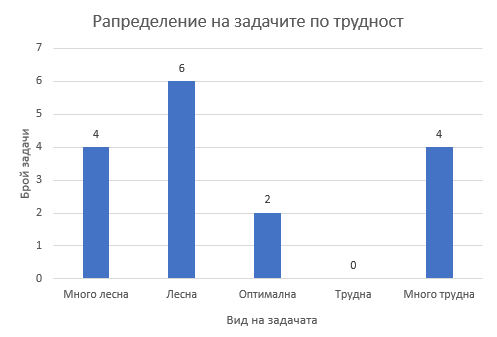
\includegraphics[width=\linewidth]{resources/trudnost.png}
    \caption{Разпределение на задачите по групи}
\end{figure}

\subsection{Коефициент на дискриминация (разграничителна сила)}
Коефициентът на дискриминация показва колко дадена задача различава учениците с висок резултат на теста от тези с нисък. За да се определят учениците от т.нар. силна група и  слаба група разглеждаме процентилите, в които попадат - преди 27-мия процентил (вкл. и 27-мия) са слабата група, а след 73-тия процентил (вкл. и 73-мия) са силната.

Силната група се състои от 8 ученици, слабата също.

Формираме коефициента като от броя на вярно отговорилите от силната група извадим броя на вярно отговорилите от слабата група.

\begin{itemize}
    \item Много добра разграничителна способност - 4
    \item Добра - 1, 5, 9, 11, 16
    \item Средна - 2, 3, 6, 10,
    \item Ниска - 7
    \item Много ниска - 8, 12-15
\end{itemize}
Средната дискриминация е 0.2, което е сравнително ниско.

Минималната дискриминация е -0.14 (зад. 15), което е много лошо - слабите ученици отговарят "по-вярно"  от силните ученици. А маскималния коефициент 0.63 е на зад. 4, което е добра разграничителна способност (всичко над 0.25 е добра способност).

Повечето задачи са концентирани в категорията добри или средни - с малко редакция можем да постигнем по-добро разграничение. Относно задачите с много нисък резултат - можем да ги преформулираме/сменим отговори или премахнем изцяло.
\begin{figure}[H]
    \centering
    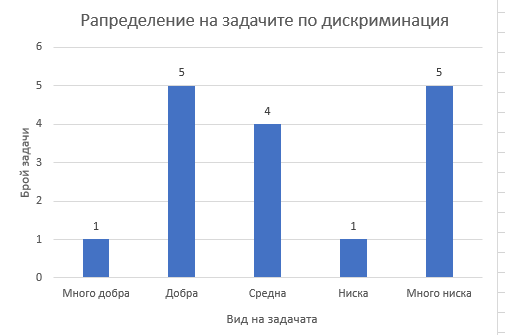
\includegraphics[width=\linewidth]{resources/diskrimination.png}
    \caption{Анализ на разграничителната сила}
\end{figure}

\subsection{Коефициент на корелация с общия бал}
Стистика, която отразява по-пълно взаимодействието от коефициента на дискриминация е този на корелация с общия бал, защото се вземат предвид резултатите на всички ученици.
\begin{itemize}
    \item Много добра разграничителна способност - 4, 16
    \item Добра - 1, 3, 5, 11
    \item Средна - 2, 6, 7, 9
    \item Ниска - 10
    \item Много ниска - 8, 12, 15
\end{itemize}
Прави впечатление, че имаме проблем с корелацията на задачи 13 и 14 - на едната никой не е отговорил вярно, а на другата всеки, което от своя страна не ги прави подходящи задачи.
\begin{figure}[H]
    \centering
    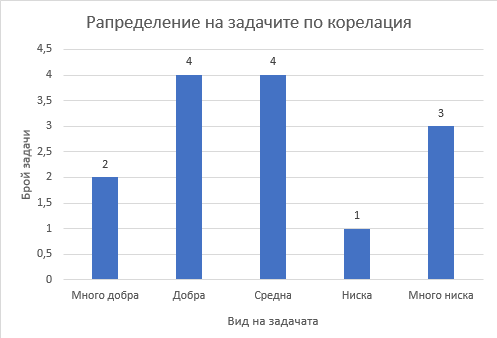
\includegraphics[width=\linewidth]{resources/korelaciq.png}
    \caption{Анализ на корелацията}
\end{figure}

\subsection{Анализ на дистракторите}
Подобно на коефициента на дискриминация се изчислява и разграничителната сила на дистракторите. Като съобразяваме, че всъщност стойностите са с обратно значение. Добър дистрактор е този с отрицателен коефициент, защото учениците от слабата група го отбелязват, но от силната - не.
\begin{figure}[H]
    \centering
    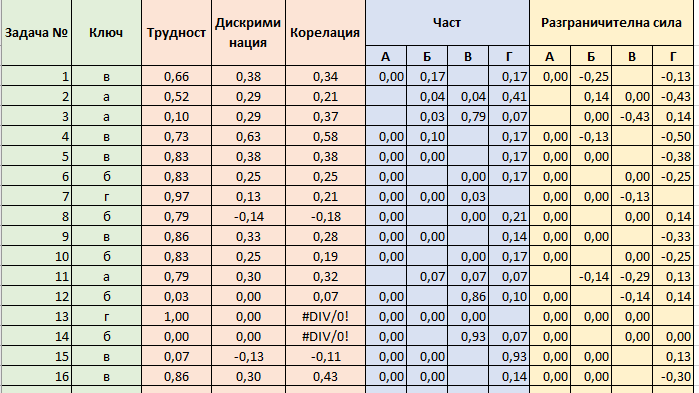
\includegraphics[width=\linewidth]{resources/distraktori.png}
    \caption{Анализ на дистракторите}
\end{figure}
Забелязваме, че част от дистракторите имат отрицателен коефициент, което е желаният ефект. Лош факт обаче е, че имаме много с разграничителна сила 0.

Дистрактор Б на задача 2, дистрактор Г на задачи 8, 11, 12 и 15 са с положителни коефициенти, което насочва вниманието към тях - вероятно трябва да бъдат преработени или преформулирани.

\subsection{Валидност на теста}
Отговаряме на въпроса: Измерва ли теста това, което претендира, че измерва?

Основните видове валидност са съдържателна, критериална, конструктна и външна.
\begin{itemize}
    \item Съдържателна валидност - задачите в теста са подходящо подбрани спрямо съдържателната рамка
    \item Критериалната валидност - според външен критерий
    \item Конструктната валидност - тестът измерва заложените за измерване знания, умения
    \item Външната валидност - визията на теста, подредба на задачи, отговори и форматиране
\end{itemize}
Валидността на тест, всъщност, се определя чрез експертна оценка.

\subsection{Надеждност на теста}
Надежността на тест определя колко точно е измерването, което целим да направим - до каква степен може да очакваме повтаряемост на резултатите.

Може да се определя по няколко начина:
\begin{itemize}
    \item Корелационна матрица
    \item Разделяне на теста на 2 части - ще разделим на четни и нечетни
    \item коефициента алфа на Кронбах
\end{itemize}
Търсения ефект е голям коефициент на надеждност (близък до 1). Тогава можем да претендираме за близост до реалния бал.
\begin{figure}[H]
    \centering
    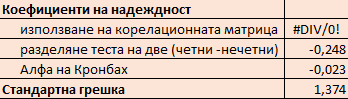
\includegraphics[width=\linewidth/2]{resources/nadezhdnost.png}
    \caption{Надеждност на теста}
\end{figure}
Използвайки коефициента на алфа на Кронбах получаваме стойност, която е по-малка от 0.75, значи не можем да твърдим, че тестът ни е надежден.

За действителния бал имаме:
\begin{figure}[H]
    \centering
    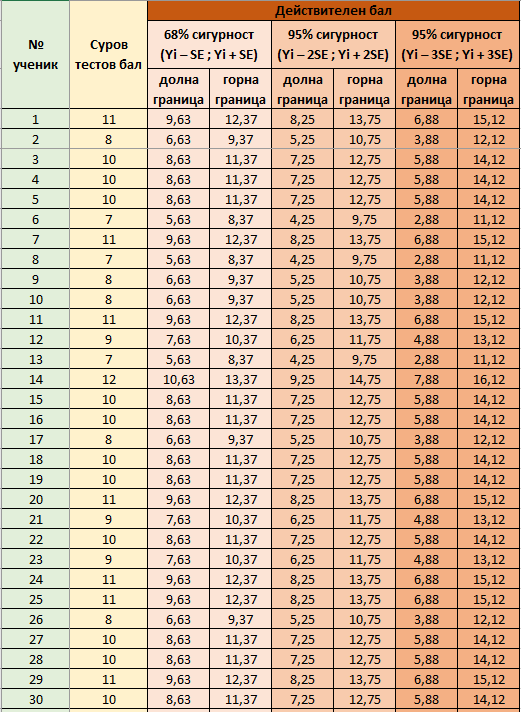
\includegraphics[width=\linewidth]{resources/deistvitelen-bal.png}
    \caption{Действителен бал}
\end{figure}

\section{Оценяване}
Ще използваме оценяване съобразено с характеристиките на теста. Искаме да намерим $k, l$, т.ч.:
\begin{equation}
    y = kx + l
\end{equation}
където $y$ е оценката на ученикът, а $x$ е броя решени задачи. За да определим $k, l$ трябва последователно да определим долна и горна граница на тестовия бал:
\begin{itemize}
    \item Долна граница - трябва да намерим теоретичната граница за налучкване (в нашия случай 4) и да прибавим стандартното отклонение (1.36) - получаваме 5
    \item Горна граница - допускаме т.нар "грешки по невнимание"  -  в нашия случай 1. Значи ученик трябва да е постигнал 15 или 16 верни отговора за отличен.
\end{itemize}
Сега търсим правата $y = kx + l$ минаваща през $\langle 5, 3 \rangle$ и $\langle 15, 6\rangle$ - такава права е единствена. $k = 0.3$ и $l = 1.5$.

В крайна сметка оценката се получава по формулата:
\begin{equation}
    G(x) = \begin{cases}
        2          & , x < 5            \\
        0.3x + 1.5 & , 5 \leq x \leq 14 \\
        6          & , x \geq 15
    \end{cases}
\end{equation}
При тази схема 19 ученици получават Добър 4 и 11 Мн. Добър 5. Нямаме отличници и нямаме ученици с нисък резултат.

Ако искаме да разграничим малко повече учениците можем да използваме норма базирана на характеристиките на учениците, когато 3ма ученици ще получат Среден 3, 19 - Добър 4, 7 - Мн. Добър 5 и един отличник.

\section{Извод}
Анализът на теста показва, че има възможност за подобрение при дистракторите и трудността на въпросите. Имайки предвид, че тестът се е оказал труден за учениците, резултатите показват, че са се справили със задоволителни резултати. Не можем обаче да извадим много добър извод за това, над какво трябва да се обърне внимание при работа с учениците, тъй като имаме въпроси с не много добра разграничителна способност.